\chapter{Layers}

\pagestyle{fancy}
\fancyhf{}
\fancyhead[OC]{\leftmark}
\fancyhead[EC]{\rightmark}
%\renewcommand{\footrulewidth}{1pt}
\cfoot{\thepage}

%%%%%%%%%%%%%%%%%%%%%%%%%%%%%%%%%%%%%%%%%%%%%%%%%%%%%%%%%%%
%%%%%%%%%%%%%%%%%%%%%%%%%%%%%%%%%%%%%%%%%%%%%%%%%%%%%%%%%%%

The term layer is given to each sheet of data mapped on the canvas.\\
The world map is a layer. The open street map is another layer.\\
We will be adding a few more layers to this QGIS project: location of headquarters will be another layer. So will the number of crimes per LSOA.\\

The order in which they exist in the \textit{Layers} panel will determine the order in which they are drawn.\\

Each layer can have it's own projection, but the software can re-project each layer onto the chosen project projection. More on this later.\\

\section{Attribute table}

Each vector layer has it's own attribute table.\\

If the layer contains point data, each row in the attribute table will correspond to a point on the map. Similarly, if the layer contains polygon data, each row in the attribute table will correspond to a polygon on the map. The World layer contains polygons - as you can see in the map canvass.\\

To open a layer's \textit{attribute table}, select the relative layer in the \textit{Layers Panel}, and then click	\begin{tabular}{@{}c@{}}
\includegraphics[width=4ex]{images/attribute_table_icon.png}\end{tabular}
, or right click on layer name in the \textit{Layers Panel} and select \textit{Open Attribute Table}. Take note of the other functionality available in this list.

\begin{figure}[!h]
	\centering
	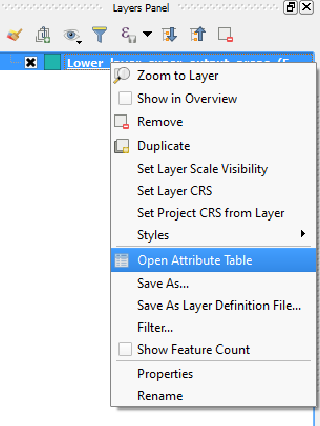
\includegraphics[width=0.3\textwidth]{images/right_click_layername_cropped.png}
	\caption{Right click on later name in Layers panel}
	\label{ft_fig_firstfig3}
\end{figure}

Can sort the data (like in excel) by clicking on the title row. Variables (columns) are referred to as \textit{fields} in GIS software. And rows as \textit{features}.\\

\begin{figure}[!h]
	\centering
	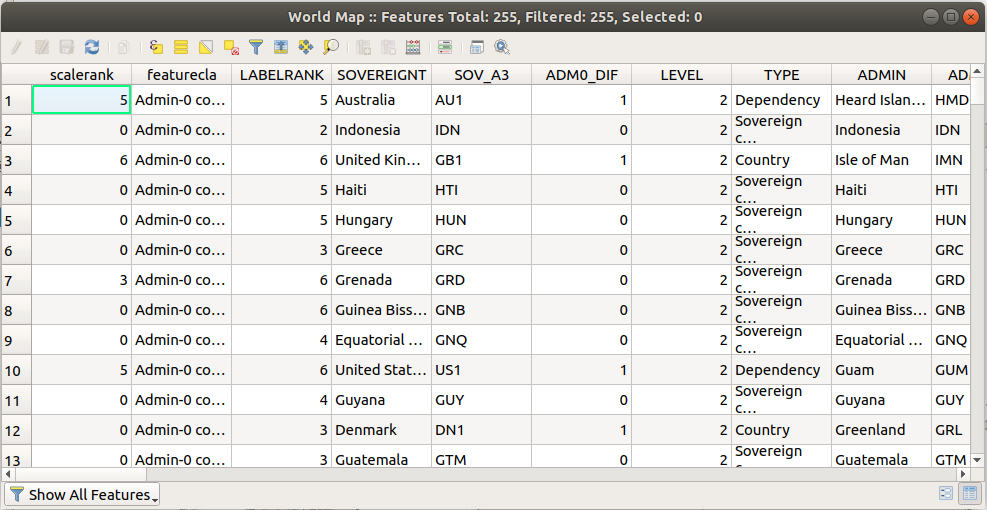
\includegraphics[width=0.6\textwidth]{images/world_attribute_table.png}
	\caption{Attribute table for World layer}
	\label{ft_fig_firstfig3}
\end{figure}

\subsection{Relationship between the attribute table and the map canvas}

\subsubsection{From attribute table to map canvas}
Can select row(/s) in attribute table and see where they are in the map canvas (they become highlighted in yellow on the map).\\

Select a row (polygon) in the attribute table. Notice the \textit{Attribute table} window title reports the number of total features, and any selected.\\

\begin{figure}[!h]
	\centering
	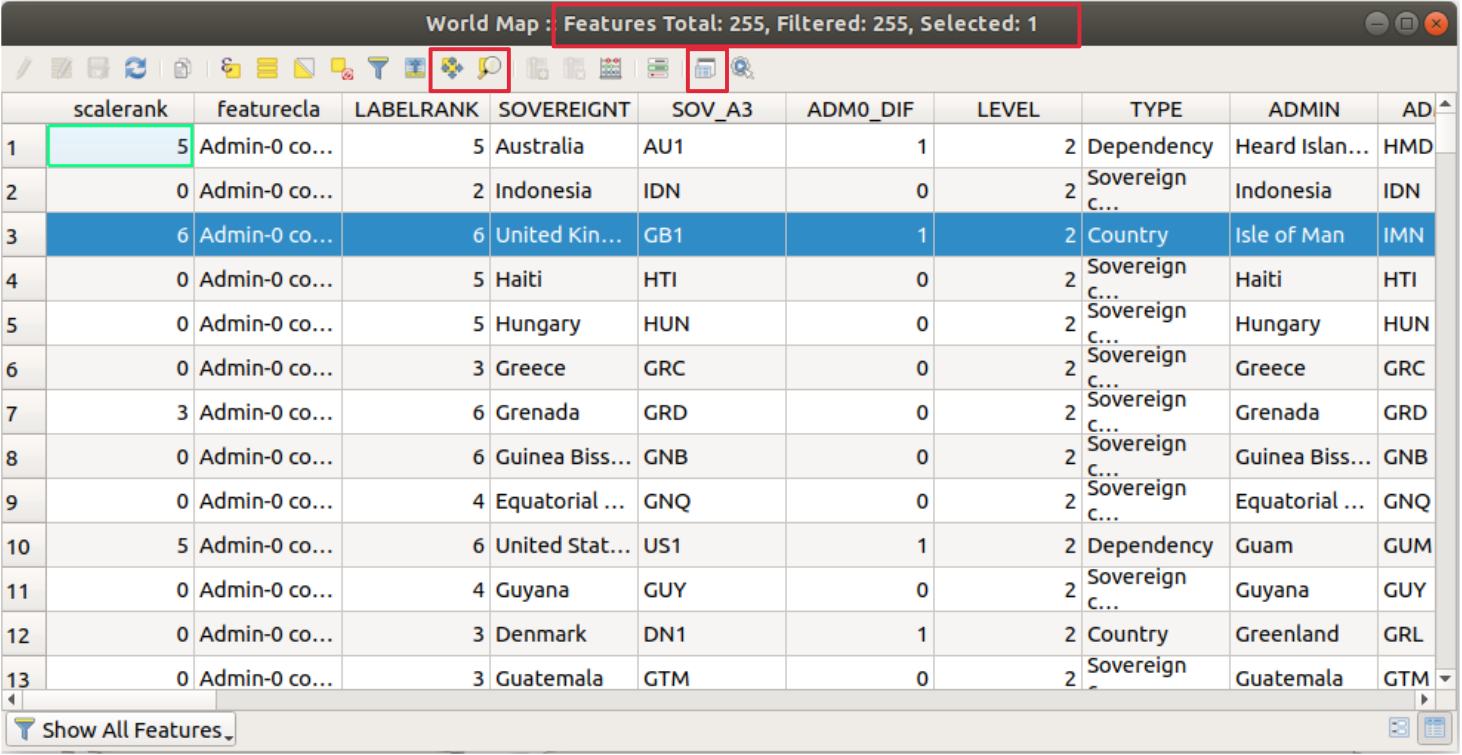
\includegraphics[width=0.55\textwidth]{images/world_attribute_table_select1_redbox.png}%stop_search_at_tbl_select_6_features_redbx.png}%attribute_table_top_rows.png}
	\caption{World attribute table with 1 feature selected. Red boxes highlight:1) Number of features selected 2) Map navigation function buttons 3) Dock attribute table icon}
	\label{ft_fig_firstfig3}
\end{figure}

TIP: We can dock the attribute table to the main window, so we can see both the map canvas and the attribute table 
\begin{tabular}{@{}c@{}}
\includegraphics[width=4ex]{images/dock_attribute_table_icon.png}\end{tabular}\\

Sometimes we can not instantly see where the selected feature(s) are on our map. Use the map navigation function buttons: \textit{Pan to selected} \& \textit{Zoom to selected}. These function buttons are in the Attributes \& Map Navigation toolbars, and in the Attribute Table title bar. For some cases, need to press this button a couple of times for it to take effect. Icons that contain \textbf{\textcolor{yellow}{yellow}} refer to functions that act on selected features.

\begin{figure}[!h]
	\centering
	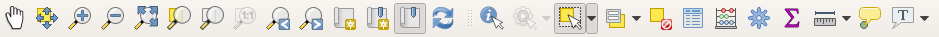
\includegraphics[width=1\textwidth]{images/attribute_and_map_navigation_toolbars_icons.png}
	\caption{Function buttons in the Attributes \& Map Navigation toolbars}
	\label{ft_fig_firstfig3}
\end{figure}

Here we see the world layer zoomed in on the Isle of man.\\

\begin{figure}[!h]
	\centering
	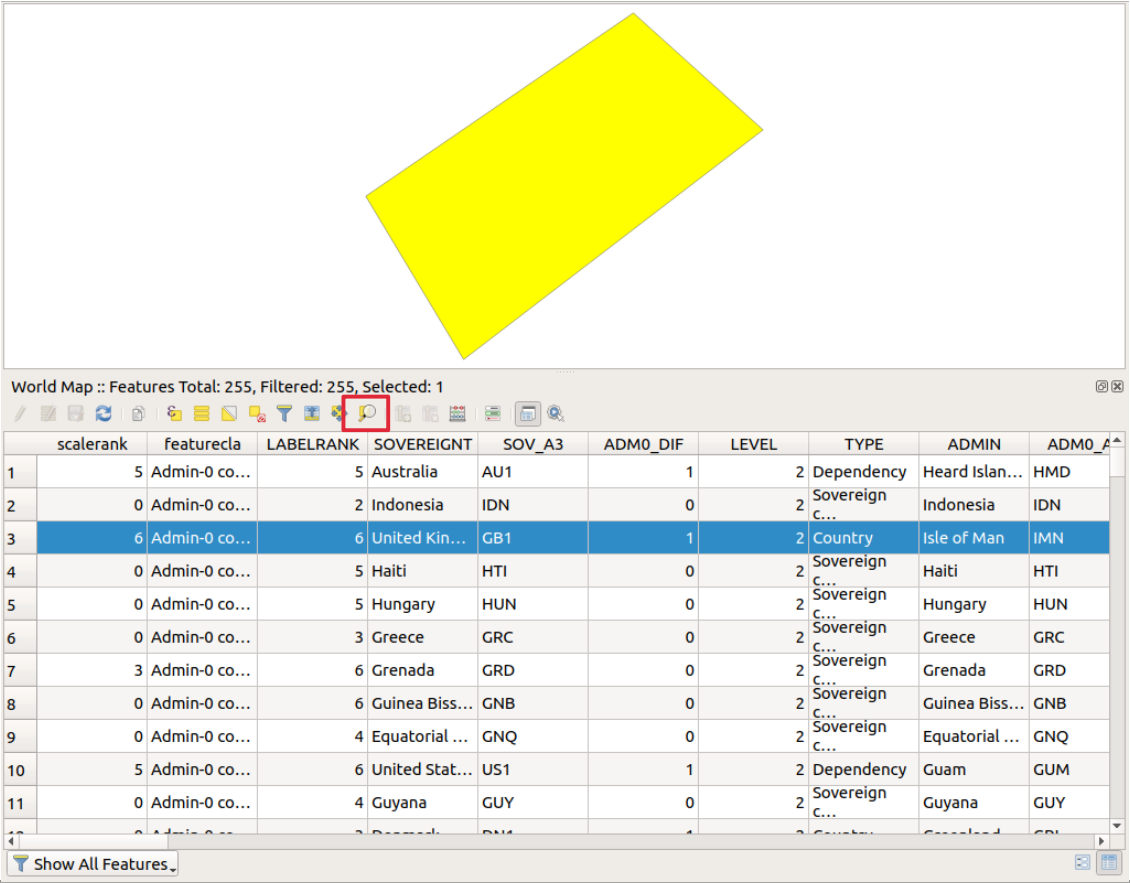
\includegraphics[width=0.8\textwidth]{images/world_map_1_select_zoom.png}
	\caption{World layer zoomed in on selected feature (Isle of man)}
	\label{ft_fig_firstfig3}
\end{figure}

Deselect features from all layers
\begin{tabular}{@{}c@{}}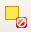
\includegraphics[width=4ex]{images/deselect_features_icon.png}\end{tabular}
and zoom full (to the shapefile layer)     
\begin{tabular}{@{}c@{}}
\includegraphics[width=4ex]{images/full_zoom_icon.png}\end{tabular}
.

\subsubsection{Moving the other way: from map canvas to attribute table using the \textit{Identify Feature} tool}

This function will only work on the top layer (as in the \textit{Layers Panel}, even if the top layer is unselected.

Click the \textit{Identify Feature} icon 
\begin{tabular}{@{}c@{}}
\includegraphics[width=4ex]{images/identify_feature_icon.png}\end{tabular}

Click on a feature (polygon). Information about that feature (polygon) will be displayed in the \textit{Identify Results Panel}, this is essentially the values of the fields in the layer's \textit{Attribute Table}):  

\begin{figure}[!h]
	\centering
	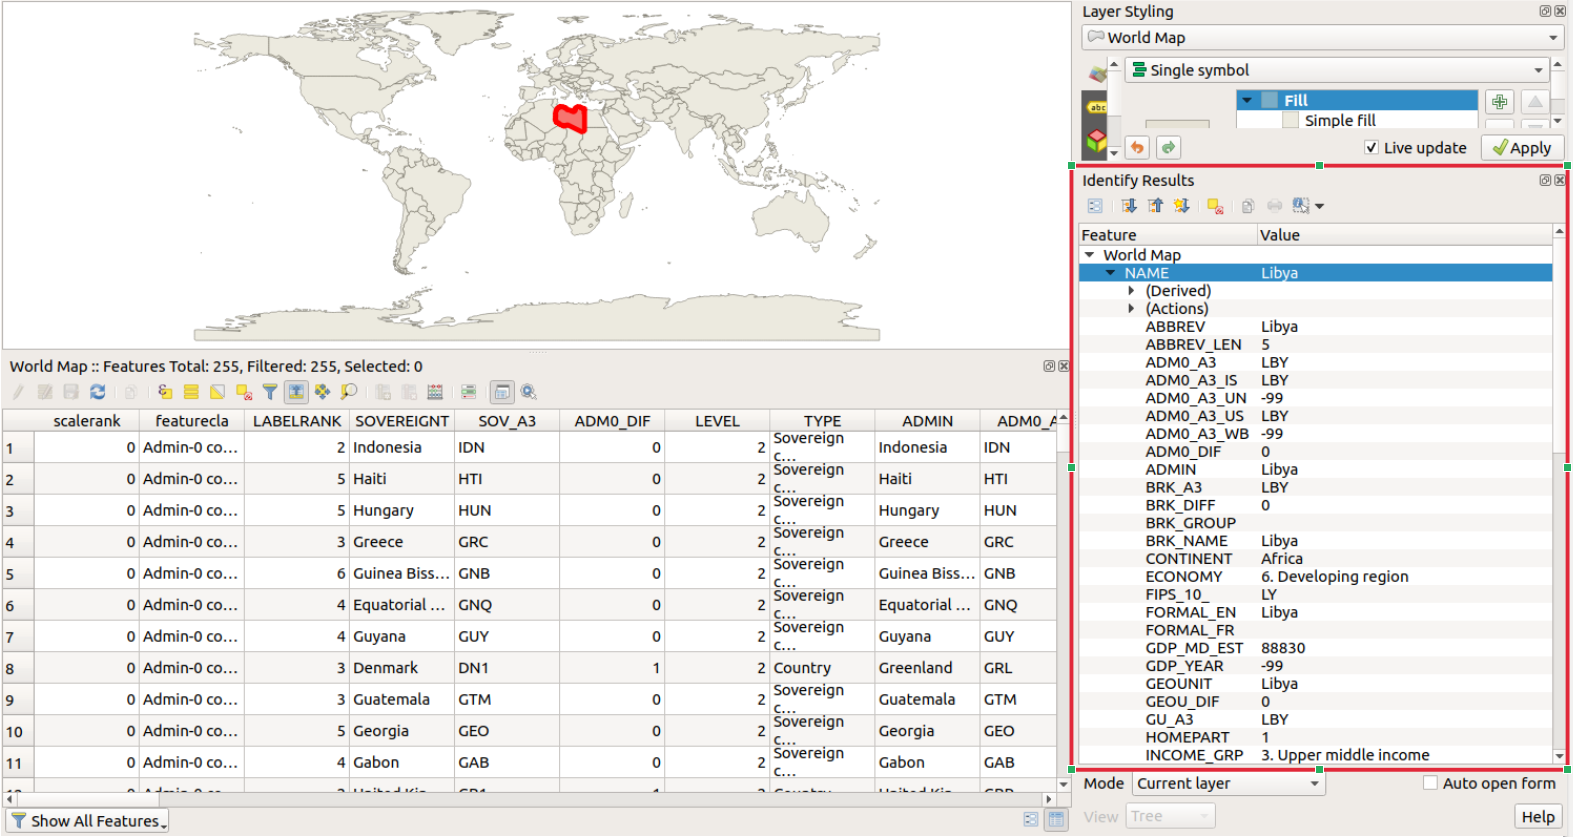
\includegraphics[width=0.6\textwidth]{images/world_identify_feature.png}%identify_feature_window.png}
	\caption{Identify Feature tool for a polygon in the world layer}
	\label{ft_fig_firstfig3}
\end{figure}

\subsubsection{From map canvas to attribute table using the \textit{Select Feature(s)} tool}

Alternatively, can select multiple features (polygons) on the map using the \textit{Select Feature(s)} tool, the icon is in the top toolbar
\begin{tabular}{@{}c@{}}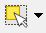
\includegraphics[width=4ex]{images/select_features_by_polygon_icon.png}\end{tabular}
, (right click to end selection) and view their field values in the \textit{Attribute Table} by moving the related rows to the top:
\begin{tabular}{@{}c@{}}
\includegraphics[width=4ex]{images/move_selection_to_top_icon.png}\end{tabular}. This is a live update feature, each time you select a different polygon(s), the corresponding row(s) will move to the top of the attribute table. Works the best with the \textit{Attribute table} docked. Make sure the \textit{Attribute table} is scrolled to show the top rows.\\

\begin{figure}[!h]
	\centering
	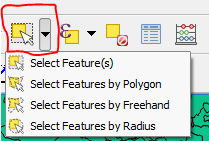
\includegraphics[width=0.35\textwidth]{images/select_features_by_polygon_dropdown.png}
	\caption{Select feature(s) tool options}
	\label{ft_fig_firstfig3}
\end{figure}

\begin{figure}[!h]
	\centering
	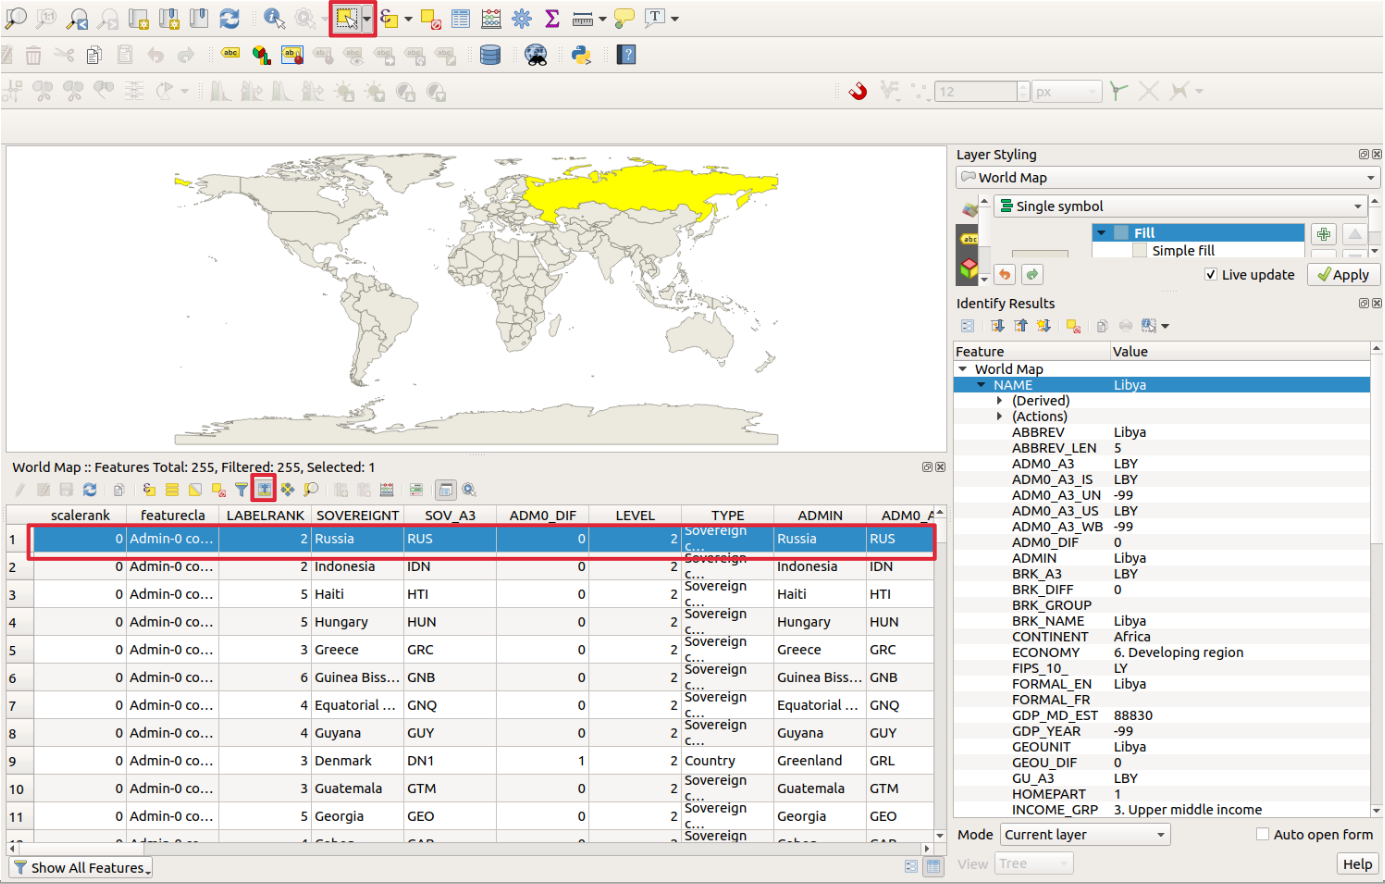
\includegraphics[width=0.85\textwidth]{images/world_select_features_to_top.png}
	\caption{Select features on map, and move those features to the top of the attribute table}
	\label{ft_fig_firstfig3}
\end{figure}

We will learn more about attribute tables throughout this tutorial.\\

Let's now close the attribute table (x in top right of attribute table window) and deselect features from all layers
\begin{tabular}{@{}c@{}}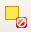
\includegraphics[width=4ex]{images/deselect_features_icon.png}\end{tabular}
\null\newpage

\section{Layer Properties window}

Most of the work we will do with our layers can be initiated through the \textit{Layer Properties} window.

To open the Layer Properties window, double click on the layer name in the Layers panel. Can also right click on layer name in \textit{Layers} panel $\rightarrow$ Properties.

The LHS tabs on the Layer Properties window:

\begin{enumerate}
	\item
	Information: Summary of the layer data
	\item
	Source: Change the Layer Name (what is used in the Layer Panel), Coordinate reference system
	\item
	Symbology: Style your layer using data from the Attribute table (can also use Layers Styling panel).
	\item
	Labels: Add labels to the layer, using text fields from the Attribute table  (can also use Layers Styling panel).
	\item
	Diagrams: Add pie chart. Text or histograms to your maps. Be careful of overcrowding your map -  only include this if your layer contains few well spaced polygons.
	\item
	3D view: If your data contains height information, this can incorporate it into the map. We’ve yet to use this.
	\item
	Source Fields: View and edit the fields in the attribute table.
	\item
	Attributes Form
	\item
	Joins: Add spatial data to the layer. Requires a common field in both files (the layer’s Attribute table, and the new data), with a unique code for each polygon.
	\item
	etc...
%	Auxiliary Storage
%	\item
%	Actions
%	\item
%	Display
%	\item
%	Rendering
%	\item
%	Variables
%	\item
%	Metadata
%	\item
%	Dependencies
%	\item
%	Legend
%	\item
%	QGIS Server
%	\item
%	Digitizing
\end{enumerate}

\begin{figure}[!h]
	\centering
	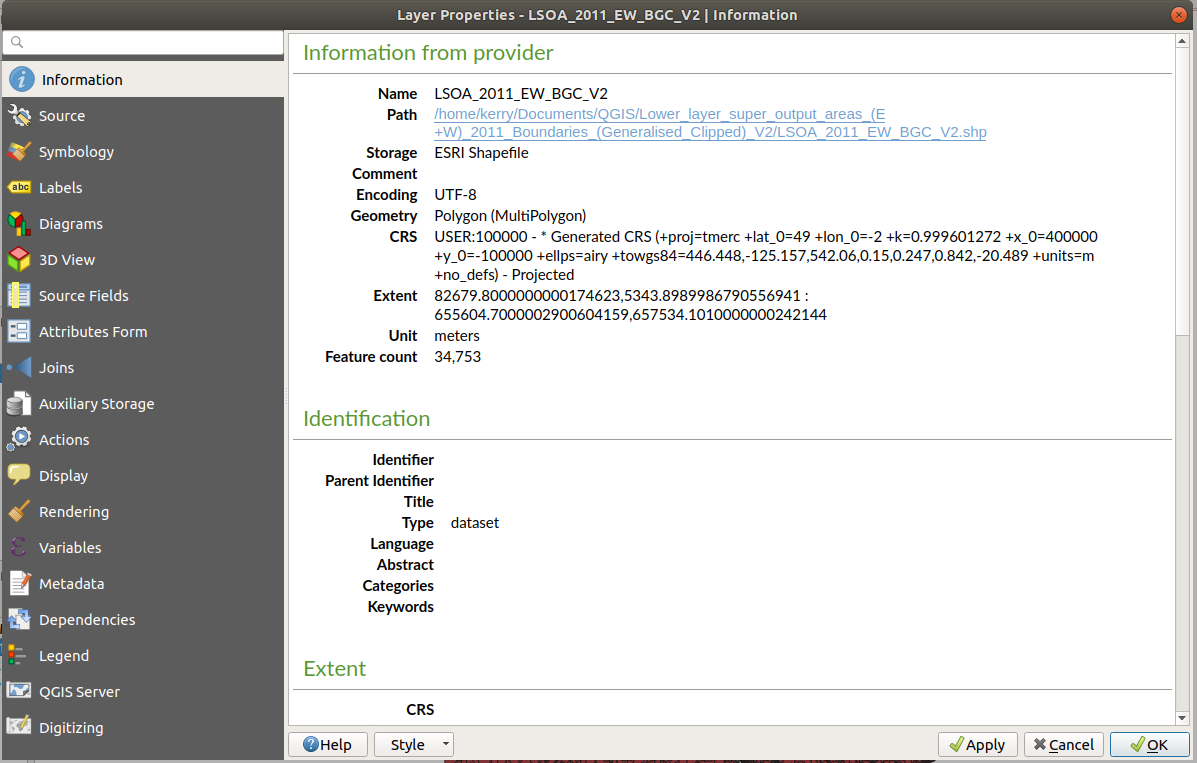
\includegraphics[width=0.8\textwidth]{images/layer_properties_window.png}
	\caption{Layer properties window}
	\label{ft_fig_firstfig3}
\end{figure}


%\section{Other functionality accessed by right click on layer name}
%\begin{enumerate}
%	\item
%	Duplicate layer
%	\item
%	Remove layer
%	\item
%	Rename layer
%	\item
%	Zoom to layer
%	\item
%	Open attribute table
%	\item
%	Export
%	\item
%	Move to top
%\end{enumerate}

%%%%
Let's now save our project
\begin{tabular}{@{}c@{}}
\includegraphics[width=4ex]{images/save_project_icon.png}\end{tabular}.\\

Close QGIS and reopen. Your project will show in the recent projects window (can select this here), or once QGIS is open use browse panel, or menu, or icon on toolbar \begin{tabular}{@{}c@{}}
\includegraphics[width=4ex]{images/open_project_icon.png}\end{tabular}. As with all programs, I'd recommend to save your work frequently.